\documentclass{article}
\usepackage[T1]{fontenc}
\usepackage{lmodern}
\usepackage{graphicx}
\usepackage{amsmath,amssymb}
\usepackage[a4paper,margin=2cm]{geometry}
\usepackage[absolute,overlay]{textpos}
\setlength{\TPHorizModule}{1mm}
\setlength{\TPVertModule}{1mm}
\usepackage[indonesian]{babel}
\usepackage{hyperref}
\setlength{\emergencystretch}{2em}
% unit: Halaman 33

\begin{document}

% === Halaman 33 (llm) ===

\vspace{215.03mm}

Plain-image \vspace{10mm} Cipher-image

% deskripsi: Gambar asli (plain-image) yang menampilkan beberapa kapal nelayan di pelabuhan dengan latar belakang mercusuar.
% bbox normalisasi: [0.0550, 0.1060, 0.4720, 0.8430]
\begin{textblock*}{87.57mm}(11.55mm,31.48mm)
\noindent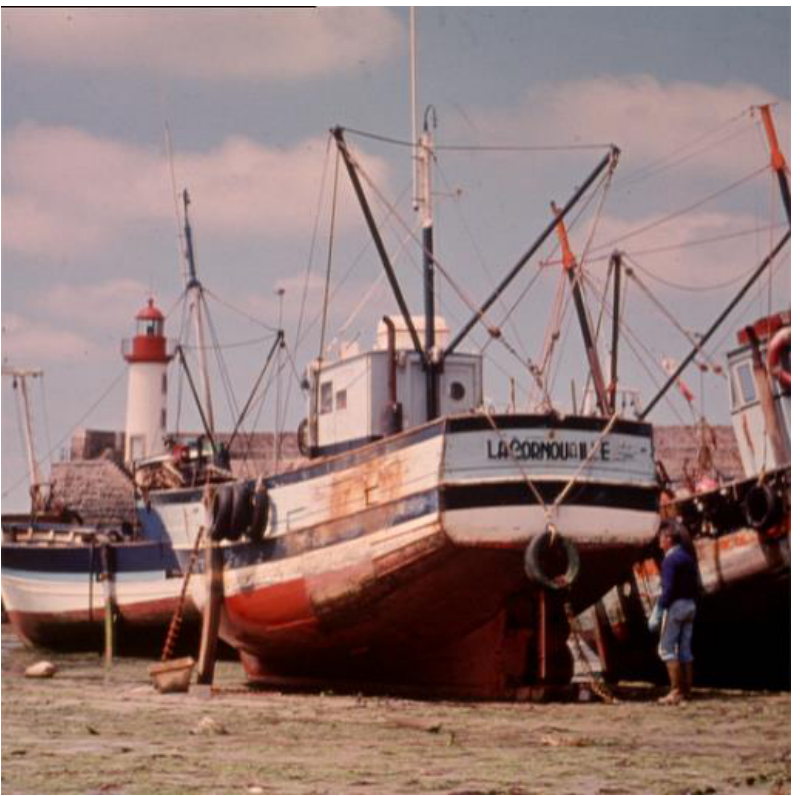
\includegraphics[width=87.57mm,height=218.89mm]{../../images/llm/page_033_img_01.png}%
\end{textblock*}

% deskripsi: Gambar terenkripsi (cipher-image) yang terlihat seperti noise acak berwarna-warni.
% bbox normalisasi: [0.5050, 0.1060, 0.9160, 0.8300]
\begin{textblock*}{86.31mm}(106.05mm,31.48mm)
\noindent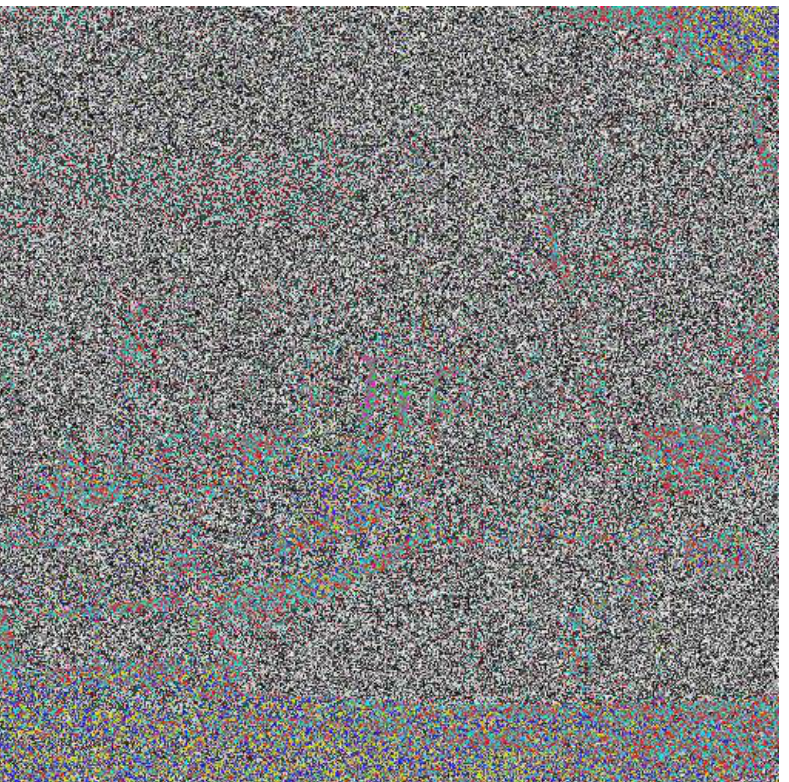
\includegraphics[width=86.31mm,height=215.03mm]{../../images/llm/page_033_img_02.png}%
\end{textblock*}

\end{document}
